%%%%%%%%%%%%%%%%%%%%%%%%%%%%%%%%%%%%%%%%%%%%%%%%%%%%%%%%%%%
\begin{frame}[fragile]\frametitle{My Talk at Nodes 2024 \ldots}
\begin{columns}
    \begin{column}[T]{0.6\linewidth}
		\begin{itemize}
		\item Computing Midcurve of a Thin Polygon for Mechanical Engineering
		\item Session Track: Data Science
		\item 12:30 pm - 1:00 pm November 7
		\item {\it 

Calculating physical product design is a complicated problem. Existing models provide rough examples in reasonable times but still require weeks of manual correcting. This presentation explores how graphs can help mechanical engineering by modeling geometric polygonal figures into a graph representation. Neural networks can then train and learn from examples provided to compute the midcurve of a thin polygon, becoming a graph-to-graph operation akin to an encoder-decoder problem.}
		\end{itemize}
    \end{column}
    \begin{column}[T]{0.4\linewidth}
		\begin{center}
		
\includegraphics[width=0.8\linewidth,keepaspectratio]{mynodes2024qr}
		\end{center}	
		
		{\tiny (QR by https://www.the-qrcode-generator.com/)}
		
		\begin{center}
		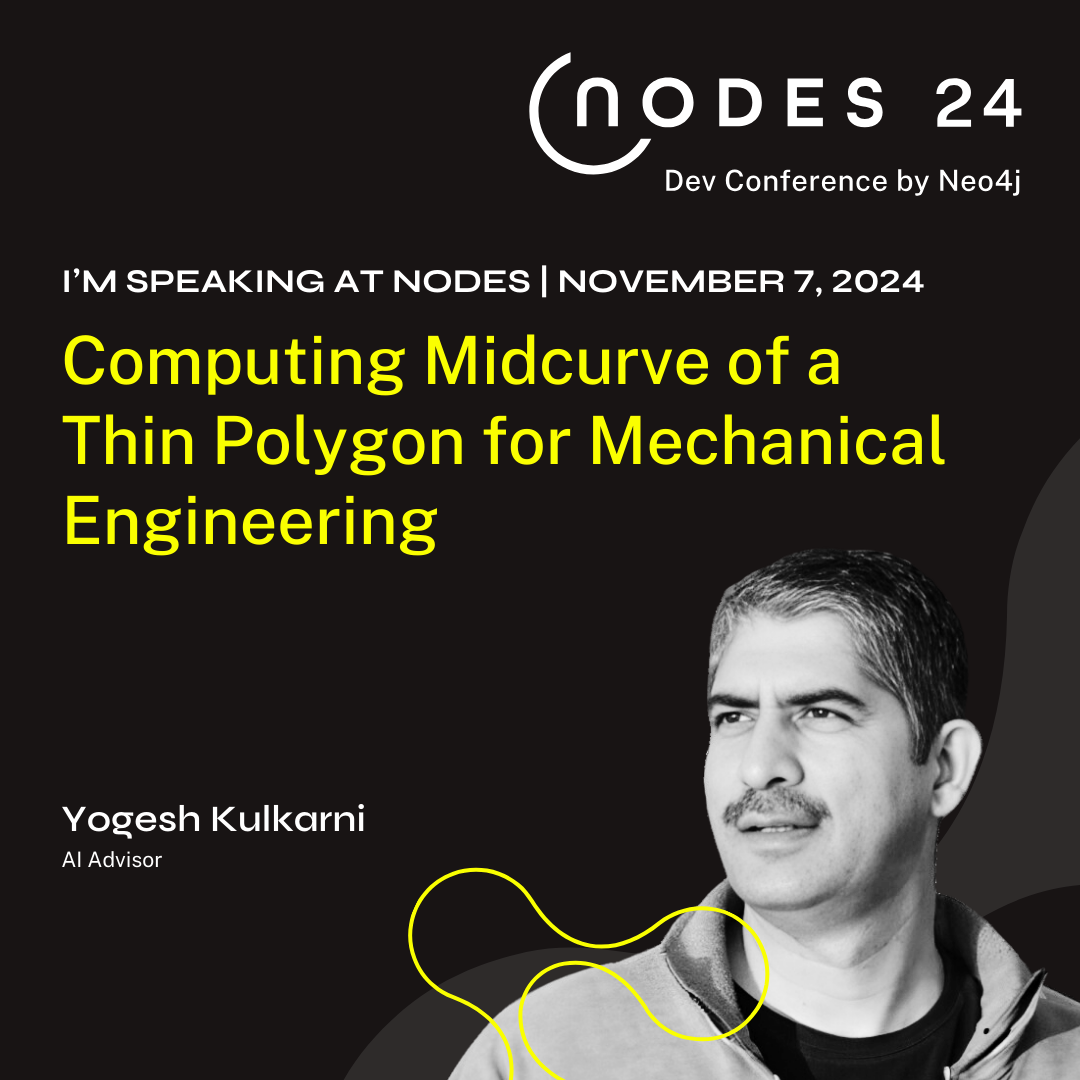
\includegraphics[width=0.6\linewidth,keepaspectratio]{Nodes24_kulkarni-speakercard}
		\end{center}			
    \end{column}
  \end{columns}
\end{frame}